\documentclass[11pt,a4paper]{jsarticle}
\usepackage{amsmath,amssymb,amsthm}
\usepackage[dvipdfmx]{graphicx}
\numberwithin{equation}{section}

\newtheorem{assumption}{Assumption}[section]
\newtheorem{proposition}[assumption]{Proposition}
\newtheorem{theorem}[assumption]{Theorem}
\newtheorem{exercise}{Exercise}[section]

\begin{document}

\setcounter{section}{11}
\section{一般状態空間モデルにおける応用的な分析例}

\subsection{構造変化の考慮}
本章では\textgt{構造変化}を伴う時系列データとして,再びナイル川の流量に関するデータについて検討を行う.
このデータにおいて,アスワン (ロウ) ダムの建設に伴う1899年からの流量急減を精度よく考慮するのが,本章の検討目的となる.
検討のステップとして,まず\textgt{変化点}が既知の場合を復習してから,変化点が未知の場合に拡張を図る.
検討にあたり,データのプロットを再掲する.
\begin{center}
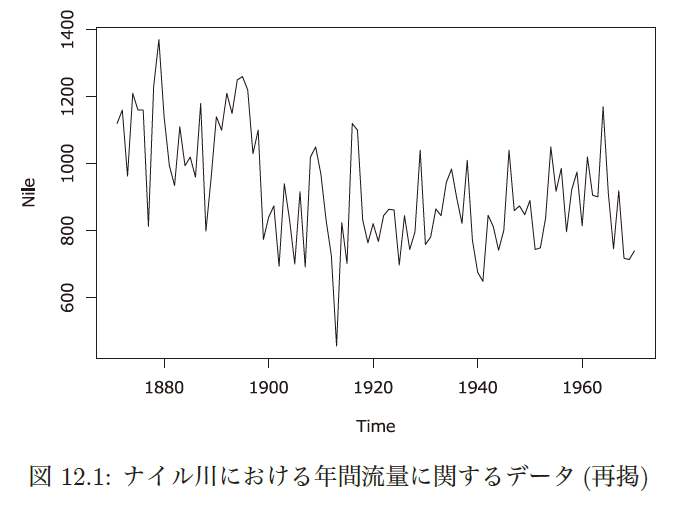
\includegraphics[width=10cm]{img/Figure12_1.png}
\end{center}

構造変化における変化点の検出は\textgt{異常検知}の一種でもあり,従来からさまざまな手法が検討・提案されている.
最近では,Rで使えるライブラリ [105–108] もいくつか存在している.
本章では変化点が既知の場合の別アプローチとし,ローカルレベルモデルの状態雑音を時変で考える方法について検討する.
パラメータを時変で考えると,構造変化への追従性を高めることができる.
本書ではこれまでパラメータは基本的に時不変と考えてきたが,以下では時変の場合も考える.
なお,本書では以降,パラメータが時変・時不変であることを,単に時変・時不変と呼ぶことにする.

またこの時変の状態雑音の考え方を踏まえて,変化点が未知の場合にも対応できるように拡張を図る.
具体的にはこのために,状態雑音に裾の厚い分布を適用する.
このようにすると,状態雑音はまれにとても大きな値をとることになる.
状態雑音は状態の時間的な変化に許容されるひずみを意味するため,その値がまれにとても大きな値をとるということは,状態の値が突然大きく変化する状況を適切に説明できることに繋がる.

以上の検討における解法としては,変化点が「既知」の場合にはカルマンフィルタを,変化点が「未知」の場合にはMCMC・粒子フィルタを適用する.
これらの結果を比較するために,条件を合わせて固定区間平滑化を考えることとする.

さらに本章の最後では,未知の変化点を実時間で検出する方法を検討する.

\subsection{カルマンフィルタによるアプローチ (変化点は既知)}
本節ではカルマンフィルタを用いて,構造変化における既知の変化点を適切に考慮する方法について説明する.

\subsubsection{これまでに検討した時不変のモデル}
まず比較対象として,これまでに検討した時不変のローカルレベルモデルの結果を振り返る.
このローカルレベルモデルは,(8.9), (8.10) 式で次のように定義されていた.
\begin{align}
x_t
& =
x_{t-1} + w_t, & w_t & \sim \mathcal{N} (0, W), \\
y_t
& =
x_t + v_t, & v_t & \sim \mathcal{N} (0, V).
\end{align}
この場合の分析はすでに「8.2 例: ローカルレベルモデルの場合」で確認した.
コードについては割愛するが,平滑化分布の平均値の結果を再掲する.
\begin{center}
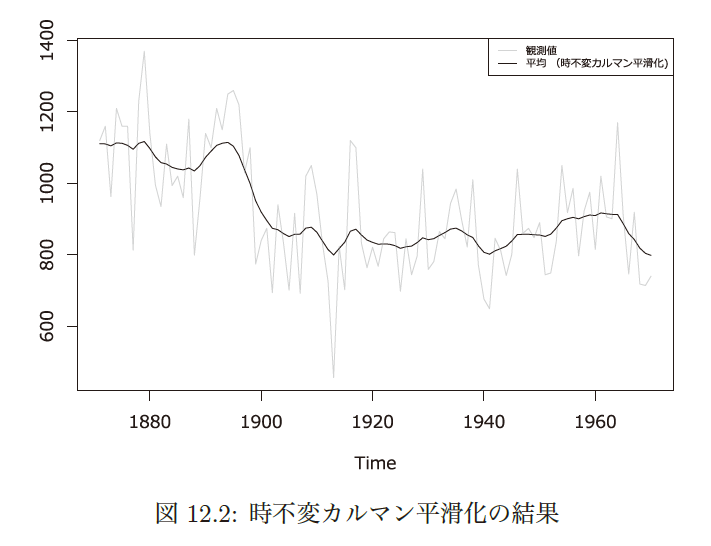
\includegraphics[width=10cm]{img/Figure12_2.png}
\end{center}

1899年の急変への追従は今一つ.
また,最尤法で特定された状態雑音の分散$W$は1468.432,観測雑音の分散$V$は15099.8となっている.
実データが対象なためこれが正解というわけでもないが,本書ではこの結果を時不変なモデルの結果に関する目安として考えることとする.

\subsubsection{線形・ガウス型状態空間モデルにおいて先見情報を活用する}
ローカルレベルモデルの状態雑音に工夫を施す方法を考える.
1899年の観測値の急激な変動を適切に考慮できるように,状態雑音の分散が1899年「だけ」大きくなると考える.
状態雑音の分散は時変となるが,ここでは変化点を既知のタイミングとして扱っているため,モデルは線形・ガウス型状態空間モデルのまま.
この場合のローカルレベルモデルは,次のように定義される.
\begin{align}
x_t
& =
x_{t-1} + w_t, & w_t & \sim \mathcal{N} (0, W_t), \\
y_t
& =
x_t + v_t, & v_t & \sim \mathcal{N} (0, V).
\end{align}
これらを (12.1), (12.2) 式と比べると,$W$が$W_t$となっている.
$W_t$は,$W_{1899年以外} = W$, $W_{1899年} = λ^2 W$とする.
$W$は通年で共通する時不変の値で,$λ^2$は1899年だけにかかる倍率となる.
このような時変のパラメータをもつ線形・ガウス型状態空間モデルに対するカルマンフィルタは,\textgt{時変カルマンフィルタ}とも呼ばれる.

\subsubsection{数値結果}
コードはNotebookを参照.

最尤法で特定された状態雑音の分散$W_t$は1899年以外が6.709260e-02,1899年が6.035191e+04,観測雑音の分散$V$は16301.65という結果になった.
この値を用いてカルマン平滑化の処理を行い,平滑化分布の平均値をプロットした.
\begin{center}
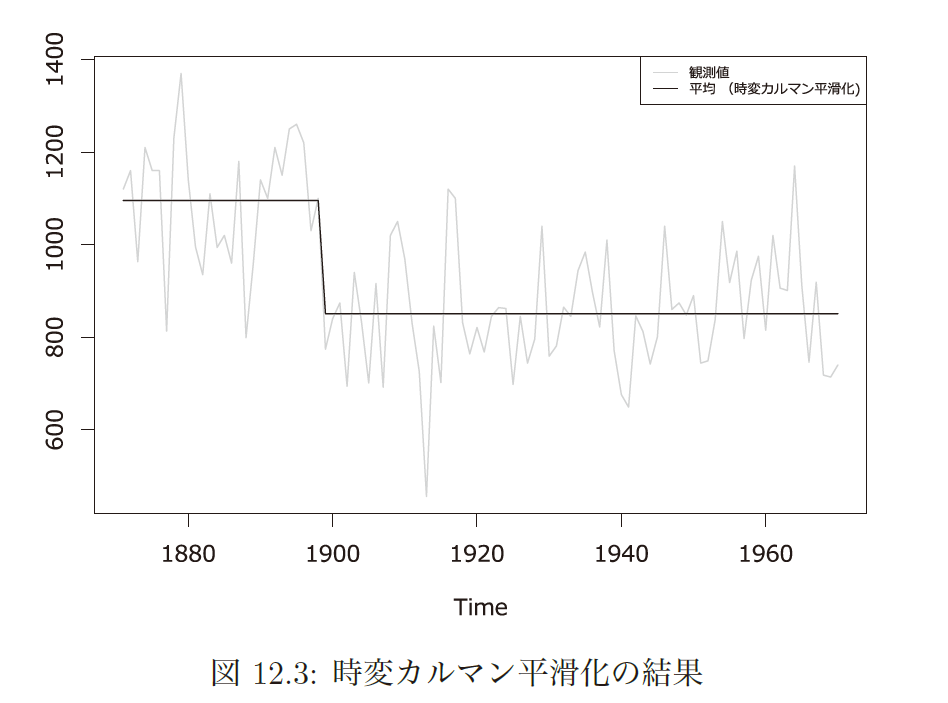
\includegraphics[width=10cm]{img/Figure12_3.png}
\end{center}

図12.3を図12.2と比較すると,1899年の急変に鋭く追従していることが分かる.
また,1899年の前後でレベルの値がほぼ一定の値になっている.
実データが対象なのでこれが正解というわけでもないが,本書ではこの結果を1899年の急変への追従に関する目安として考えることにする.

\subsection{MCMCを活用した解法によるアプローチ (変化点は未知)}

\subsubsection{これまでに検討した時不変のモデル}
比較対象として,これまで検討した時不変のローカルレベルモデルの結果を振り返る.
ローカルレベルモデルの定義は (12.1), (12.2) 式と同じだが,ここではパラメータの$W$, $V$も確率変数と考え,状態とあわせて推定を行う.
「10.5 推定精度向上のためのテクニック」での説明に基づき,まずパラメータの$W$, $V$のみMCMCを活用して推定するが,本章では状態の推定に関してFFBSは用いず,パラメータの推定結果 (平均値) をカルマンフィルタにプラグインして推定することとする.
このような簡易な方法を用いる主な理由は,続く粒子フィルタでの検討と条件をあわせるため.

パラメータの推定には,コード10.5, 10.6がほぼそのまま利用できる.
推定された状態雑音の分散$W$ (平均) は2865.51,観測雑音の分散$V$ (平均) は14606.24となった.
最尤法で特定された結果と比べると,状態雑音の分散$W$がやや大きめだが,観測雑音の分散$V$は近い値になっている.
状態に関する平滑化分布の結果は以下の通り.
\begin{center}
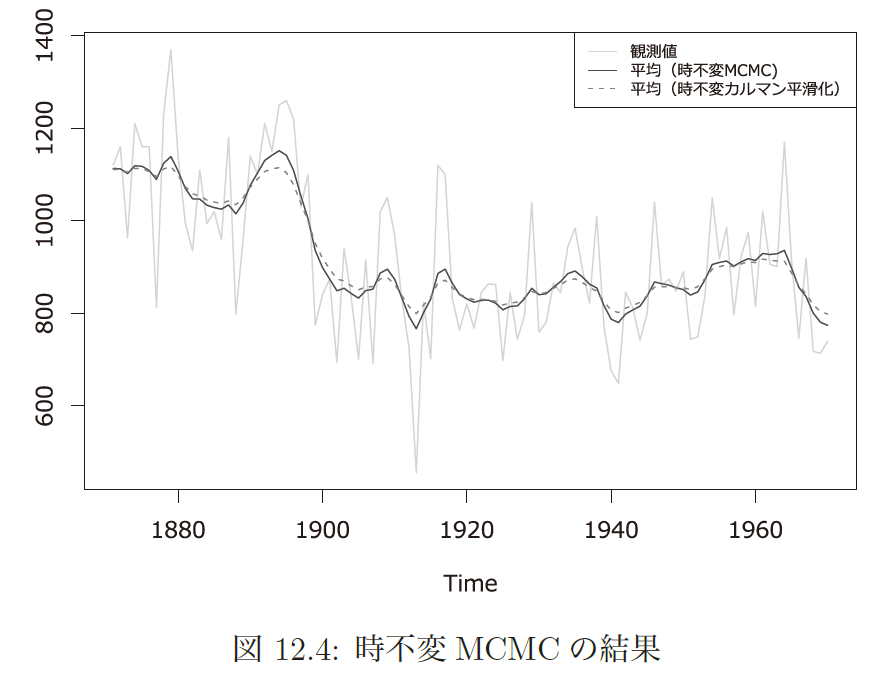
\includegraphics[width=10cm]{img/Figure12_4.png}
\end{center}

1899年の急変への追従は今一つだ.
時不変カルマン平滑化の結果と比べると,状態雑音の分散$W$の推定結果が最尤推定値より大きめだったため,全体的に変動がやや激しくなっている.

\subsubsection{一般状態空間モデルにおいて馬蹄分布を活用する}
前節では歴史上の事実という先見情報に基づいて時変のモデルを特定したが,このような情報が常に得られるとは限らない.
先見情報のない中でまれに発生する構造変化を適切に考慮するため,状態雑音に正規分布以外の分布を適用してみる.
「まれ」の程度がある程度想定のつく場合,正規分布の混合分布を適用するのもよい.
「まれ」ではあるものの程度が不明確な場合には,\textgt{裾の厚い分布}を適用するのが一般的.
よく用いられるのは,$t$分布やコーシー分布 (Cauchy distribution, 自由度1の$t$分布).

最近では裾の厚さだけでなく峰への集中度も高めた\textgt{馬蹄分布 (Horseshoe distribution)}が提案されている.
馬蹄分布は正規分布の尺度混合により,次のように定義される.
\begin{align}
馬蹄分布(中心=0, 尺度=\sigma)
& =
\mathcal{N}(0, λ_t^2 \sigma^2), \\
λ_t
& \sim
\mathcal{C}^+(中心= 0, 尺度= 1).
\end{align}
$\mathcal{C}^+$は実現値のとり得る領域を正に限定したコーシー分布であり,半コーシー分布と呼ばれる.
(12.5) 式は,正規分布の尺度 (標準偏差) に対して半コーシー分布に基づく時変倍率$λ_t$を考慮すると,その分布は馬蹄分布になることを意味する.
また(12.6) 式から,時変の倍率は通常1より小さい値をとる一方,まれに大きな値をとるため,馬蹄分布もおおむね$\sigma$より小さい値をとる一方で,まれに大きな値をとることになる.

馬蹄分布は裾の厚さに加え峰への集中度が高いという特徴により,\textgt{スパース性}を表現するのに適した分布になっている.
スパース性の表現に適した分布としてラプラス分布 (両側指数分布) もよく取り上げられるが,馬蹄分布はさらに峰への集中度が高くなっている.
コーシー分布・ラプラス分布の密度と馬蹄分布の密度を以下で比較した (全ての分布で,中心=0,尺度=1).
\begin{center}
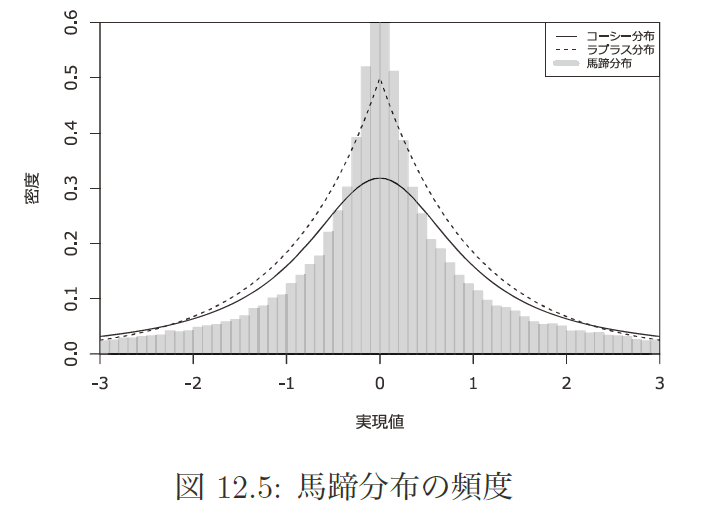
\includegraphics[width=8cm]{img/Figure12_5.png}
\end{center}


馬蹄分布は解析的な表現ができないため,サンプルサイズを50,000とした場合のシミュレーション度数を表示した.
馬蹄分布はコーシー分布・ラプラス分布と同程度の裾の厚さを保ちながら,峰への集中度が高くなっている.

馬蹄分布のもう1つの特徴は,計算上の利点にある.
正規分布の尺度混合による表現のため,条件付きで線形・ガウス型状態空間モデルが利用できる.
ただし,(12.5) 式における尺度の倍率$λ_t$が時変であるため,解法には時変のカルマンフィルタが必要になる.

馬蹄分布にはこのように魅力的な特徴があるため,状態雑音が従う分布を馬蹄分布として検討を行う.
このようなローカルレベルモデルは,次のように定義される.
\begin{align}
x_t
& =
x_{t-1} + w_t, & w_t & \sim 馬蹄分布(中心=0, 尺度=\sqrt{W}), \\
y_t
& =
x_t + v_t, & v_t & \sim \mathcal{N} (0, V).
\end{align}
(12.3), (12.4) 式と比べると,$w_t$の従う分布が正規分布から馬蹄分布に変更になっている.
このため,$w_t$は通常$\sqrt{W}$より小さい値をとるが,まれに大きな値となる.

\subsubsection{数値結果}
Notebookを参照 (次回説明します).

\end{document}
